%%%%%%%%%%%%%%%%%%%%%%%%%%%%%%%%%%%%%%%%%%%%%%%%%%%%%%
%SEC%%%%%%%%%%%%%%%%%%%%%%%%%%%%%%%%%%%%%%%%%%%%%%%%%%
\section{Introdução}

%SUBSEC%%%%%%%%%%%%%%%%%%%%%%%%%%%%%%%%%%%%%%%%%%%%%%%
\subsection{Motivação}

%FRAME%%%%%%%%%%%%%%%%%%%%%%%%%%%%%%%%%%%%%%%%%%%%%%%
\begin{frame}{Motivação}
Uso de reconhecimento facial em lojas de varejo \pause para:
\medskip
\begin{itemize}
    \item Segurança
    \pause
    \item Personalização de serviço
    \pause
    \item Marketing
    \pause
    \item Análise de sentimento
\end{itemize}
\end{frame}


%FRAME%%%%%%%%%%%%%%%%%%%%%%%%%%%%%%%%%%%%%%%%%%%%%%%
\begin{frame}
    \centerline{\noindent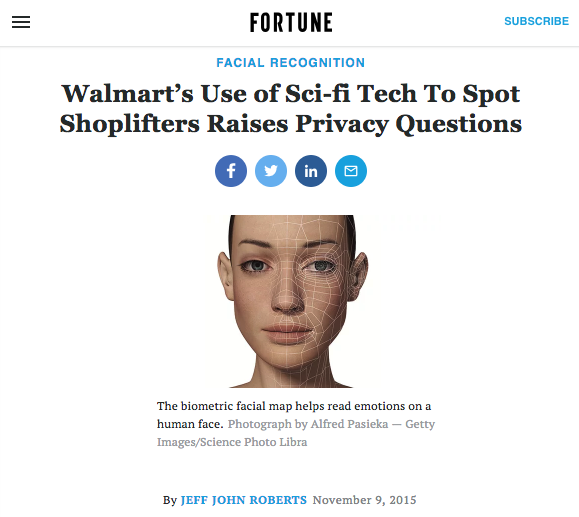
\includegraphics[width=0.8\linewidth]{Reportagem_3.png}}
\end{frame}


%FRAME%%%%%%%%%%%%%%%%%%%%%%%%%%%%%%%%%%%%%%%%%%%%%%%
\begin{frame}
    \centerline{\noindent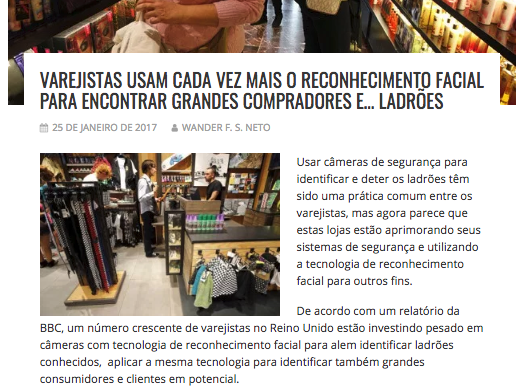
\includegraphics[width=0.8\linewidth]{Reportagem_2.png}}
\end{frame}


%FRAME%%%%%%%%%%%%%%%%%%%%%%%%%%%%%%%%%%%%%%%%%%%%%%%
\begin{frame}
    \centerline{\noindent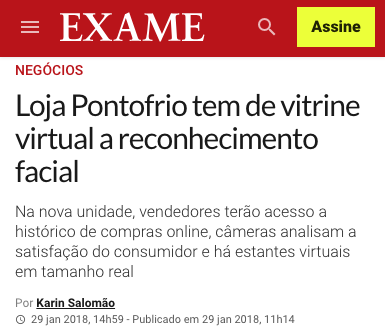
\includegraphics[width=0.8\linewidth]{Reportagem_1.png}}
\end{frame}

%FRAME%%%%%%%%%%%%%%%%%%%%%%%%%%%%%%%%%%%%%%%%%%%%%%%
\begin{frame}
    \centerline{\noindent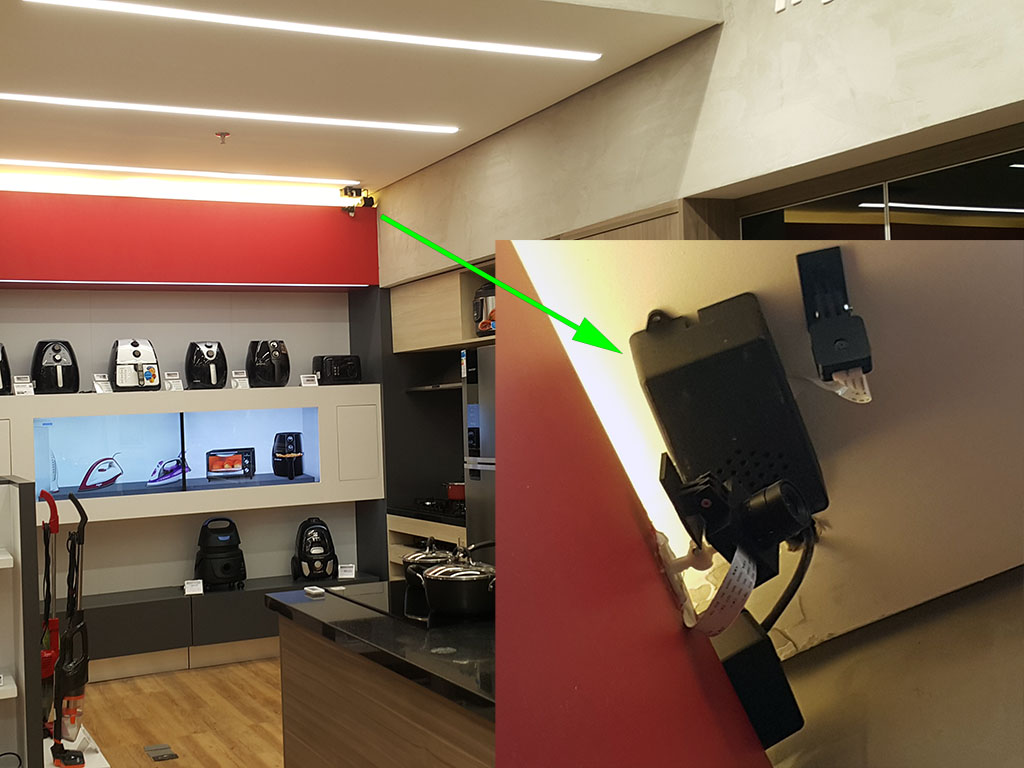
\includegraphics[width=0.8\linewidth]{imagens/ponto_frio_camera.jpg}}
\end{frame}

%SUBSEC%%%%%%%%%%%%%%%%%%%%%%%%%%%%%%%%%%%%%%%%%%%%%%%
\subsection{Objetivos}

%FRAME%%%%%%%%%%%%%%%%%%%%%%%%%%%%%%%%%%%%%%%%%%%%%%%
\begin{frame}{Objetivos}
%Os objetivos deste trabalho são:
\begin{itemize}
    \item Fornecer uma base teórica e prática para a construção de um sistema de detecção e reconhecimento facial, que será utilizado em uma loja de varejo
    \item Encontrar bibliotecas, APIs e ferramentas que auxiliem no desenvolvimento do projeto
\end{itemize}
\end{frame}


%FRAME%%%%%%%%%%%%%%%%%%%%%%%%%%%%%%%%%%%%%%%%%%%%%%%
\begin{frame}{Aplicações}
Aplicações de detecção e reconhecimento facial:
\medskip
\begin{itemize}
    \item Identificação criminal
    \item Sistemas de segurança
    \item Biometria
    \item Processamento de imagens
    \item Interação humano-computador
\end{itemize}
\end{frame}

%FRAME%%%%%%%%%%%%%%%%%%%%%%%%%%%%%%%%%%%%%%%%%%%%%%%
\begin{frame}{Exemplo}
\centerline{\noindent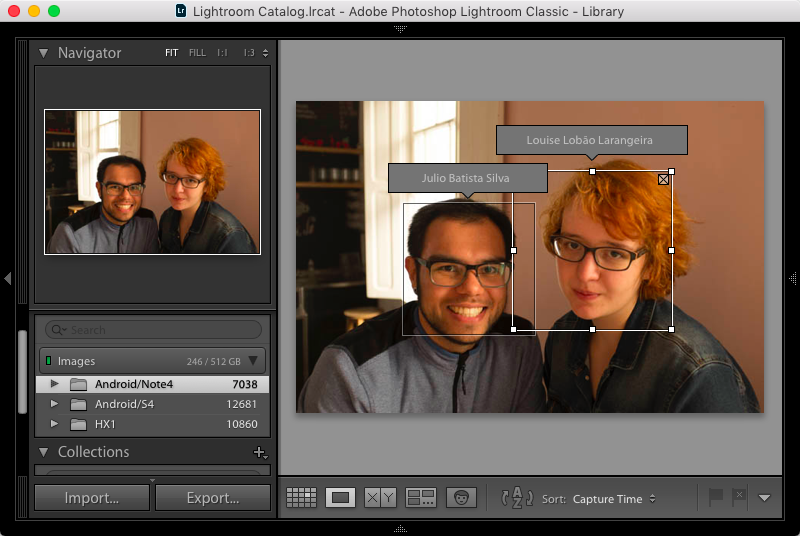
\includegraphics[width=0.9\linewidth]{lightroom_reconhecimento.png}}
\end{frame}

%FRAME%%%%%%%%%%%%%%%%%%%%%%%%%%%%%%%%%%%%%%%%%%%%%%%
\begin{frame}{Nem sempre funciona como esperado}
\centerline{\noindent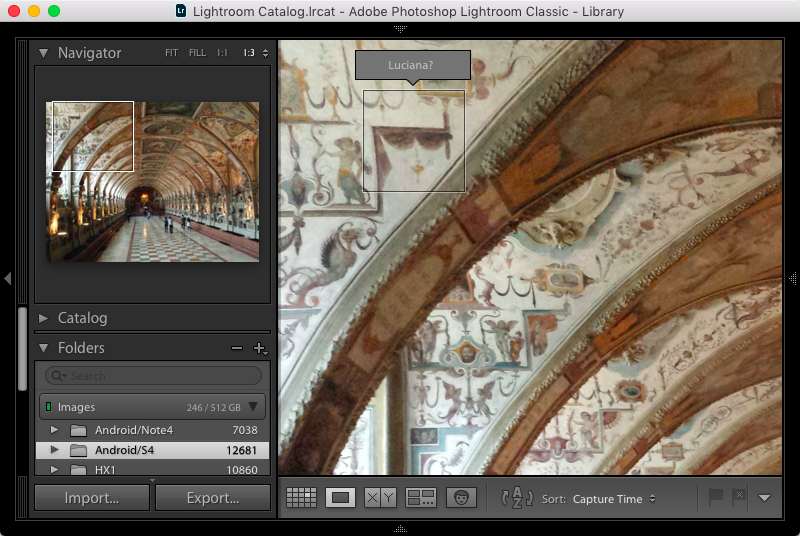
\includegraphics[width=0.9\linewidth]{lightroom_erro.png}}
\end{frame}


%FRAME%%%%%%%%%%%%%%%%%%%%%%%%%%%%%%%%%%%%%%%%%%%%%%%
\begin{frame}{Dificuldades}
\begin{overprint}
\begin{figure}
\centering

% Imagens de cima
\only<1-5>{\begin{minipage}{0.31\textwidth}
  \caption{Iluminação}
  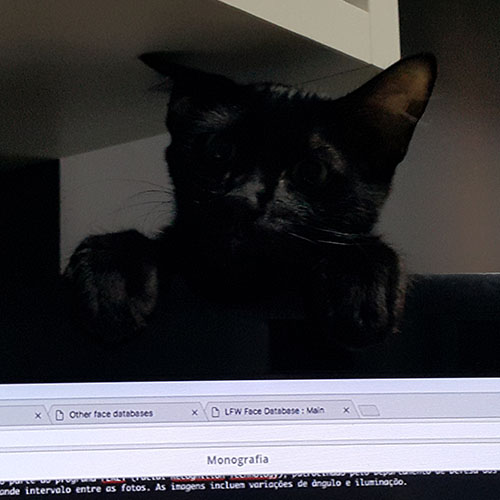
\includegraphics[width=0.8\textwidth]{imagens/iluminacao_01.jpg}
\end{minipage}}
\only<2-5>{\begin{minipage}{0.31\textwidth}
    \centering
    \caption{Pose}
    \label{fig:oclusao}
    \begin{subfigure}[t]{0.5\textwidth}
    \centering
    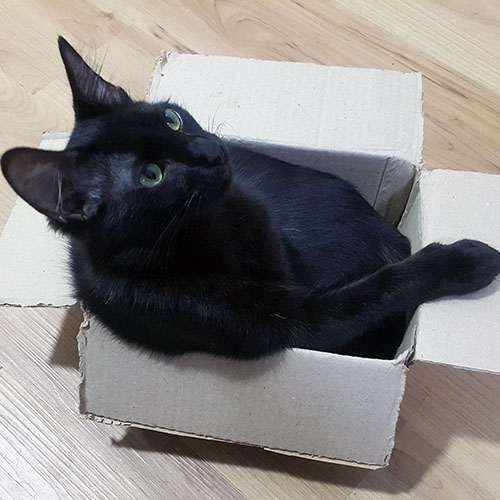
\includegraphics[width=0.8\linewidth]{imagens/pose_01.jpg}
    \end{subfigure}
    \begin{subfigure}[t]{0.5\textwidth}
    \centering
    
\includegraphics[width=0.8\linewidth]{imagens/pose_02.jpg}
    \end{subfigure}
\end{minipage}}

% Imagens de baixo
\only<3-5>{\begin{minipage}{0.31\textwidth}
    \centering
    \caption{Expressão Facial}
    \label{fig:expressao_facial}
    \begin{subfigure}[t]{0.5\textwidth}
    \centering
    
\includegraphics[width=0.85\linewidth]{imagens/expressao_01.jpg}
    \end{subfigure}
    \begin{subfigure}[t]{0.5\textwidth}
    \centering
    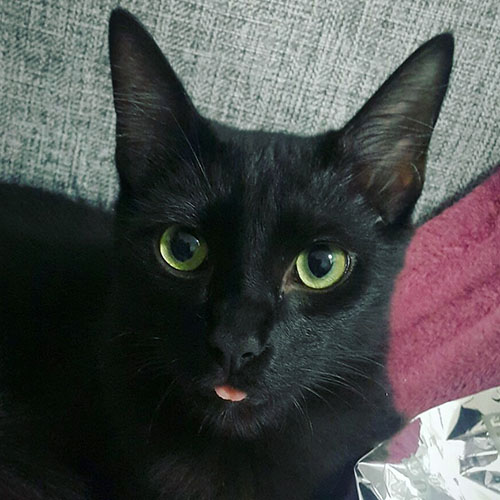
\includegraphics[width=0.85\linewidth]{imagens/expressao_02.jpg}
    \end{subfigure}
\end{minipage}}
\only<4-5>{\begin{minipage}{0.31\textwidth}
    \centering
    \caption{Oclusão}
    \label{fig:oclusao}
    \begin{subfigure}[t]{0.5\textwidth}
    \centering
    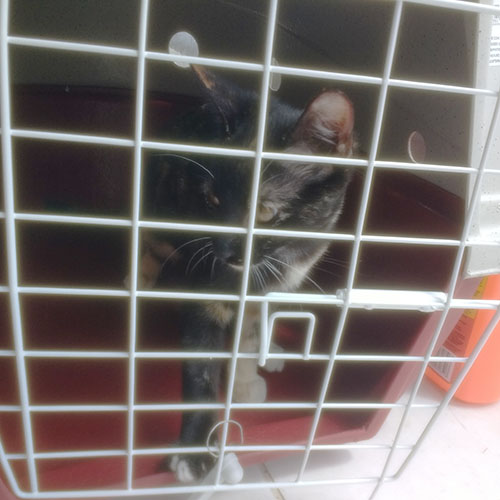
\includegraphics[width=0.85\linewidth]{imagens/oclusao_01.jpg}
    \end{subfigure}
    \begin{subfigure}[t]{0.5\textwidth}
    \centering
    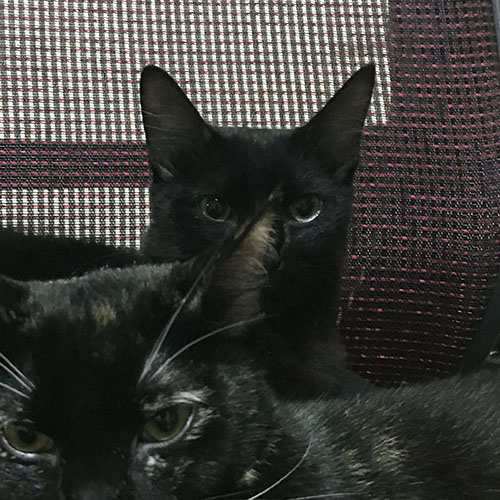
\includegraphics[width=0.85\linewidth]{imagens/oclusao_02.jpg}
    \end{subfigure}
\end{minipage}}
\only<5>{\begin{minipage}{0.31\textwidth}
    \centering
    \caption{Ponto de Vista}
    \label{fig:ponto_vista}
    \begin{subfigure}[t]{0.5\textwidth}
    \centering
    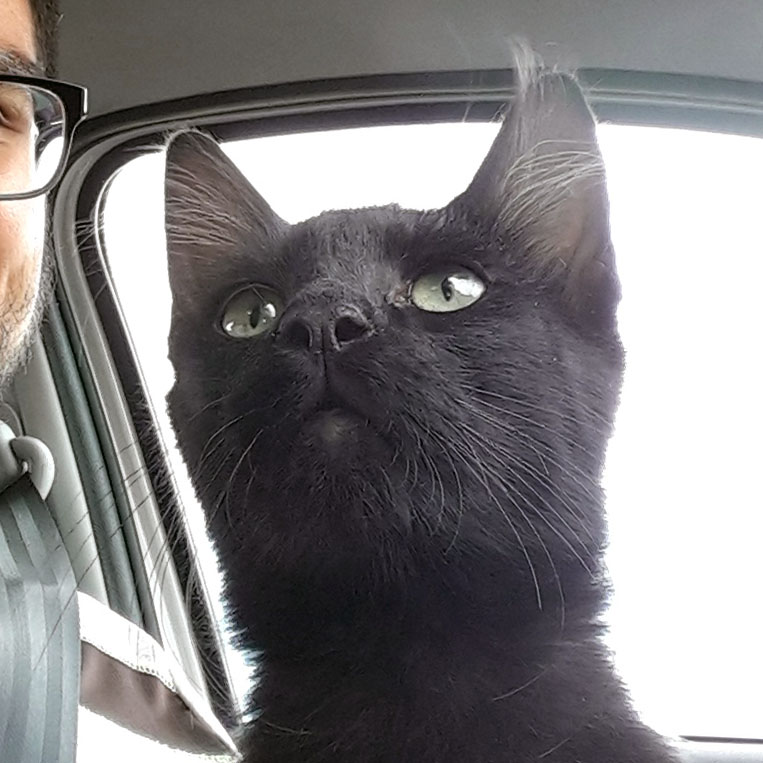
\includegraphics[width=0.85\linewidth]{imagens/ponto_vista_01.jpg}
    \end{subfigure}
    \begin{subfigure}[t]{0.5\textwidth}
    \centering
    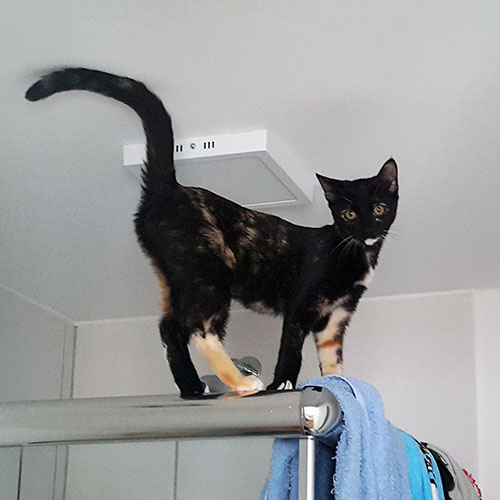
\includegraphics[width=0.85\linewidth]{imagens/ponto_vista_02.jpg}
    \end{subfigure}
\end{minipage}}
\end{figure}
\end{overprint}\end{frame}